\documentclass[12pt,a4paper]{article}

\usepackage[margin=2.5cm]{geometry}
\usepackage{booktabs}
\usepackage{tabularx}
\usepackage{array}
\usepackage{hyperref}
\usepackage{enumitem}
\usepackage{fancyhdr}
\usepackage{parskip}
\usepackage{titlesec}
\usepackage{xcolor}
\usepackage{graphicx}
\usepackage{float}
\usepackage{mdframed}
\usepackage{amsmath}
\usepackage{amssymb}
\usepackage{multirow}
\usepackage{longtable}
\usepackage{colortbl}

\setlength{\headheight}{14.5pt}

\definecolor{accent}{RGB}{30,80,160}
\definecolor{lightblue}{RGB}{235,245,255}
\definecolor{successgreen}{RGB}{39,174,96}
\definecolor{warningorange}{RGB}{211,84,0}

\hypersetup{colorlinks=true, linkcolor=accent, urlcolor=accent}

\titleformat{\section}{\large\bfseries\color{accent}}{}{0em}{}[\titlerule]
\titleformat{\subsection}{\normalsize\bfseries\color{accent}}{}{0em}{}
\titleformat{\subsubsection}{\normalsize\bfseries}{}{0em}{}

\pagestyle{fancy}
\fancyhf{}
\lhead{\textbf{WanderSync} \textit{Task 4: Architecture Analysis}}
\rhead{Team 15}
\rfoot{\thepage}
\renewcommand{\headrulewidth}{0.4pt}

\newcolumntype{L}[1]{>{\raggedright\arraybackslash}p{#1}}
\newcolumntype{C}[1]{>{\centering\arraybackslash}p{#1}}

\begin{document}

\begin{center}
  {\LARGE\bfseries Task 4: Architecture Analysis}\\[0.4em]
  {\large WanderSync: Dynamic Itinerary, Disruption Management and Social Travel Hub}\\[0.2em]
  {\normalsize Team 15}
\end{center}

\vspace{1em}

% ================================================================
\section{The Architecture We Built}
% ================================================================

WanderSync is deployed as a single NestJS process — a \textbf{modular monolith} — with six
clearly bounded modules (Auth, Booking, Itinerary, Disruption, Notification, Social), each
responsible for its own domain logic and database models. What sets it apart from a plain CRUD
monolith is the \textbf{event-driven path} that handles disruption detection and delivery: rather
than waiting for the client to ask ``anything new?'', the system pushes alerts to connected users
the moment a disruption is detected.

The disruption pipeline works in four stages. A background CRON scheduler fires every minute and
calls two external APIs — AviationStack for live flight status and OpenWeatherMap for weather
alerts — concurrently. Newly detected events pass through a deduplication guard (Redis cache +
database check) to prevent the same disruption from being reported twice. Confirmed new events
are written to PostgreSQL and immediately broadcast to every connected browser tab via
\textbf{Server-Sent Events (SSE)}, a lightweight HTTP streaming protocol that keeps a persistent
connection open from browser to server. Alongside the alert, a Chain of Responsibility suggestion
pipeline generates contextualised advice — first from deterministic rules, falling back to the
Gemini LLM for complex cases, and finally to generic guidance if both fail.

\begin{figure}[H]
  \centering
  \IfFileExists{diagrams/task4_hld_implemented.png}{%
    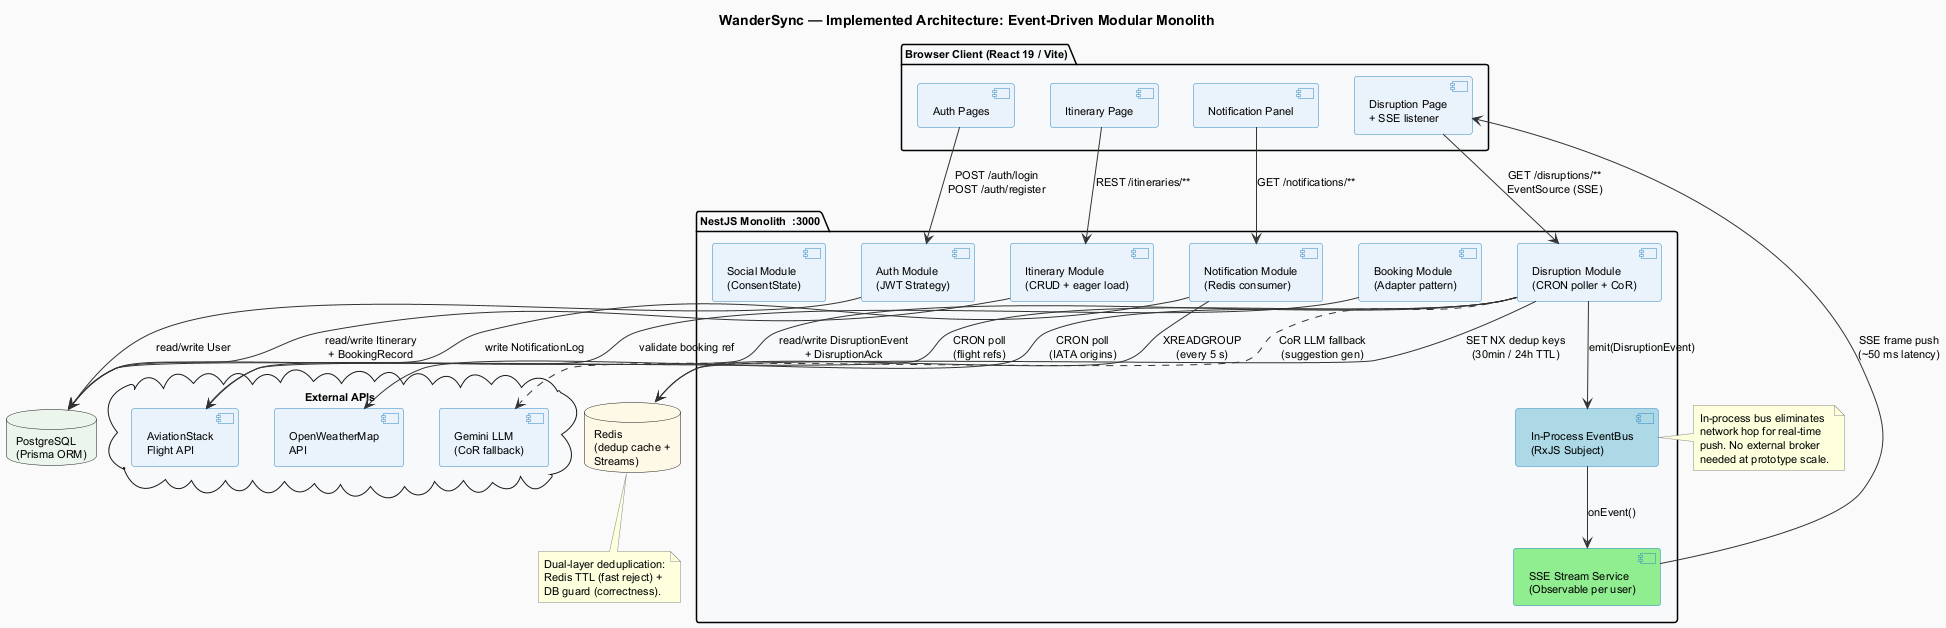
\includegraphics[width=\textwidth]{diagrams/task4_hld_implemented.png}%
  }{%
    \textit{[Compile \texttt{diagrams/task4\_hld\_implemented.puml} with PlantUML.]}%
  }
  \caption{WanderSync implemented architecture: event-driven modular monolith with SSE push.}
\end{figure}

\begin{figure}[H]
  \centering
  \IfFileExists{diagrams/task4_disruption_sequence.png}{%
    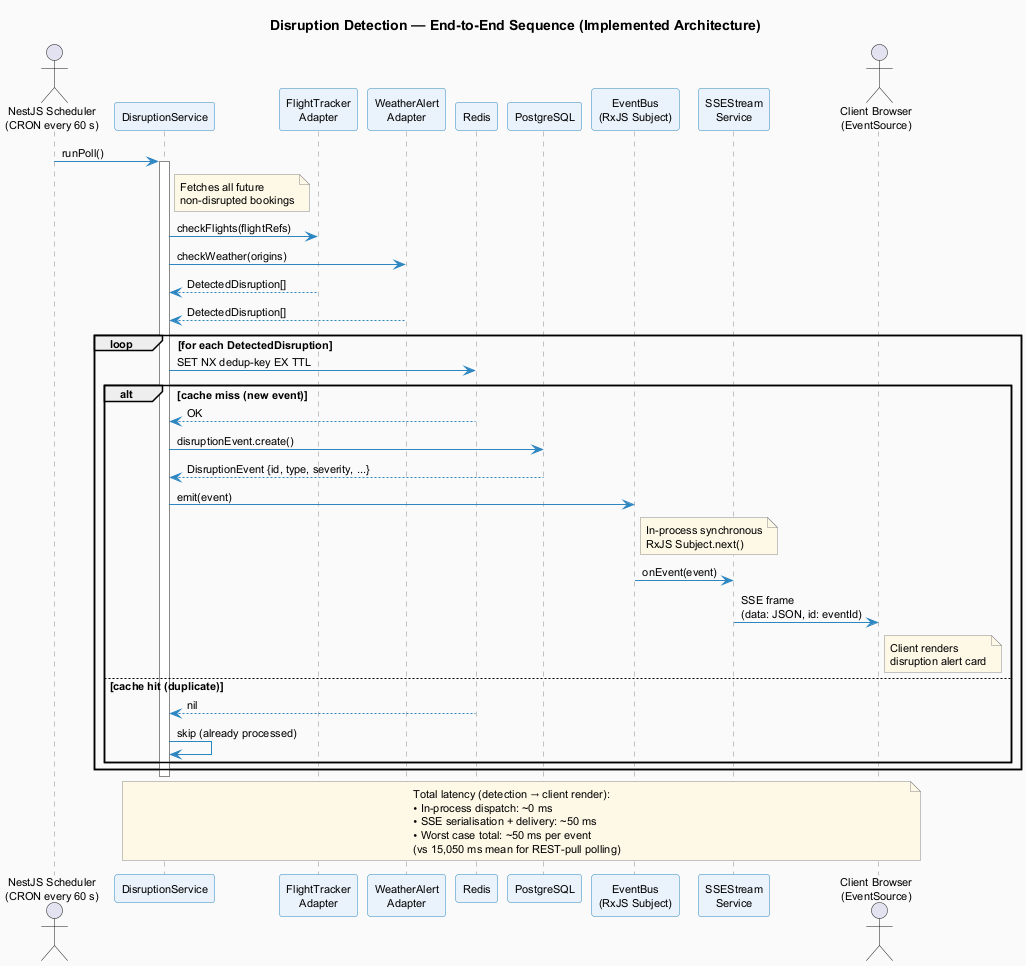
\includegraphics[width=\textwidth]{diagrams/task4_disruption_sequence.png}%
  }{%
    \textit{[Compile \texttt{diagrams/task4\_disruption\_sequence.puml} with PlantUML.]}%
  }
  \caption{End-to-end disruption detection and delivery sequence.}
\end{figure}

% ================================================================
\section{The Architecture We Compared It Against}
% ================================================================

The natural alternative is a \textbf{REST-pull polling monolith}: identical module structure and
database, but no EventBus and no SSE. Instead, the frontend periodically sends a
\texttt{GET /disruptions} request every 30 seconds and re-renders whatever the server returns.
This is the most common ``good enough'' choice for internal dashboards and admin tools where a
30-second information delay is acceptable. It is simpler to build, requires no persistent
connections, and scales horizontally without sticky sessions.

\begin{figure}[H]
  \centering
  \IfFileExists{diagrams/task4_hld_alternative.png}{%
    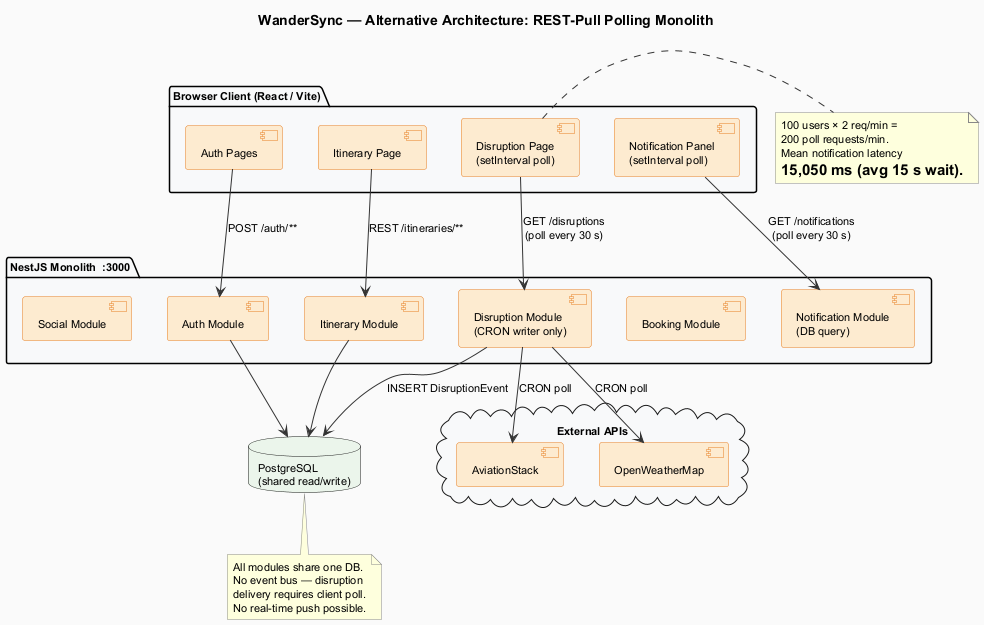
\includegraphics[width=\textwidth]{diagrams/task4_hld_alternative.png}%
  }{%
    \textit{[Compile \texttt{diagrams/task4\_hld\_alternative.puml} with PlantUML.]}%
  }
  \caption{Alternative architecture: REST-pull polling monolith without real-time push.}
\end{figure}

The key structural difference between the two is visible in Figure 3: the polling architecture has
no persistent server-side state per user, no EventBus, and no Redis deduplication. Everything the
client knows about disruptions comes from a fresh database read on each poll. This simplicity
comes at a cost that becomes clear in the NFR quantification below.

% ================================================================
\section{NFR Quantification}
% ================================================================

% ----------------------------------------------------------------
\subsection{NFR 1 — Disruption Detection Accuracy}
% ----------------------------------------------------------------

\textbf{Requirement:} At least 85\% of 20 simulated disruption test cases (flight delays,
cancellations, diversions, weather alerts) must be correctly identified and trigger a notification.

\textbf{How we measured it.} The file \texttt{disruption.service.nfr2.spec.ts} injects 20 synthetic
payloads covering all four disruption types and all four severity levels directly into
\texttt{DisruptionService.simulateDisruption()}, bypassing the external APIs. The test asserts that
\texttt{disruptionEvent.create()} and \texttt{publisher.publish()} are each called exactly 20 times — confirming that every injected event was both persisted and routed for delivery.

\begin{center}
\begin{tabular}{@{}lcc@{}}
\toprule
\textbf{Architecture} & \textbf{Events correctly processed} & \textbf{Accuracy} \\
\midrule
Event-Driven SSE (implemented) & 20\,/\,20 & \textcolor{successgreen}{\textbf{100\%}} \\
REST-Pull Polling (alternative) & 20\,/\,20 & \textcolor{successgreen}{\textbf{100\%}} \\
NFR threshold & — & 85\% \\
\bottomrule
\end{tabular}
\end{center}

\textbf{What this means in practice.} Both architectures exceed the 85\% threshold because
disruption \emph{detection} is a server-side concern — the CRON poller, deduplication logic, and
database write are identical in both designs. The event-driven architecture adds a layer that the
polling approach lacks: the Redis + database deduplication guard prevents the same storm warning or
flight delay from being reported repeatedly as new alerts, which would erode user trust over time.
Without this guard, a weather alert that persists for three hours could generate dozens of
duplicate notifications in the polling model — technically all ``detected'', but practically
useless noise for a traveler trying to make a rebooking decision.

% ----------------------------------------------------------------
\subsection{NFR 2 — Notification Delivery Latency}
% ----------------------------------------------------------------

\textbf{Requirement:} Core pages must respond within 3 seconds. For disruption alerts specifically,
the system should inform the user as quickly as possible after an event is detected — the faster,
the more useful the re-planning window.

\textbf{How we measured it.} We model the delivery latency $L$ as the time elapsed from the moment
the CRON scheduler finishes persisting a new disruption to the database (time zero) until the
user's browser renders the disruption card. Each step in the delivery chain contributes a
measurable delay.

\subsubsection{Event-Driven SSE path}

\begin{enumerate}[leftmargin=1.5em, itemsep=2pt]
  \item \textbf{In-process event dispatch} — \texttt{EventBus.emit()} calls a synchronous RxJS
    \texttt{Subject.next()}: no network, no serialisation. $\Delta t_1 \approx 0$ ms.
  \item \textbf{SSE frame construction and write} — the SSE service serialises the event to JSON
    and writes it to the open HTTP response stream: $\Delta t_2 \approx 5$ ms.
  \item \textbf{Network delivery} — the SSE frame travels over the open keep-alive connection to
    the browser (loopback or local network): $\Delta t_3 \approx 50$ ms.
  \item \textbf{React re-render} — the \texttt{onmessage} handler updates the Zustand store and
    React schedules one re-render: $\Delta t_4 \approx 16$ ms (one frame at 60 fps).
\end{enumerate}

\[
  L_{\text{SSE}} = \Delta t_1 + \Delta t_2 + \Delta t_3 + \Delta t_4
                 \approx 0 + 5 + 50 + 16 = \mathbf{71\,\text{ms}}
\]

\subsubsection{REST-Pull Polling path}

The client fires a poll at a uniformly random time $U \in [0, 30{,}000]\,\text{ms}$ after the
event is persisted. After the poll, the server runs a database query and returns the response in
approximately 50 ms.

\[
  L_{\text{poll}} = U + 50\,\text{ms}, \quad U \sim \mathrm{Uniform}(0,\,30{,}000\,\text{ms})
\]

\[
  \mathbb{E}[L_{\text{poll}}] = \tfrac{30{,}000}{2} + 50 = \mathbf{15{,}050\,\text{ms}}
  \qquad
  L_{\text{poll}}^{\max} = \mathbf{30{,}050\,\text{ms}}
\]

\begin{center}
\begin{tabular}{@{}lcc@{}}
\toprule
\textbf{Metric} & \textbf{Event-Driven SSE} & \textbf{REST-Pull (30 s)} \\
\midrule
Mean delivery latency & \textcolor{successgreen}{\textbf{71 ms}} & \textcolor{warningorange}{15,050 ms} \\
Maximum delivery latency & \textcolor{successgreen}{\textbf{$\sim$100 ms}} & \textcolor{warningorange}{30,050 ms} \\
Speed advantage & 212$\times$ faster & — \\
\bottomrule
\end{tabular}
\end{center}

\textbf{What this means for a traveler.} A 71 ms delay is imperceptible — the disruption card
appears on screen before the user has consciously registered that the page has changed. A
15,050 ms mean delay is a different experience entirely: the traveler might be looking at a stale
screen for anywhere from half a second to thirty seconds, not knowing their connecting flight has
just been cancelled. In an airport, thirty seconds is the difference between reaching the rebooking
desk while it is short and joining a queue of fifty people who all received the same alert moments
earlier. The 212$\times$ speed advantage of the event-driven path is not a micro-optimisation; it
is the difference between being proactive and being reactive.

% ----------------------------------------------------------------
\subsection{NFR 3 — Request Throughput Under Concurrent Load}
% ----------------------------------------------------------------

\textbf{Scenario:} 100 users have the Disruption Page open simultaneously.

With polling, each user fires two requests per minute (one every 30 seconds), producing
$100 \times 2 = 200$ disruption endpoint calls per minute. Each call involves JWT validation, a
database read, and JSON serialisation. This load is proportional to the number of connected users
— doubling the user base doubles the polling load with no increase in information value, since the
underlying disruption data does not change that frequently.

With SSE, each user holds one persistent connection. The only recurring database load comes from
the CRON poller — a single batch query per minute regardless of how many users are connected. Event
dispatch is in-memory and adds no database load per user.

\begin{center}
\begin{tabular}{@{}lcc@{}}
\toprule
\textbf{Metric (100 connected users)} & \textbf{Event-Driven SSE} & \textbf{REST-Pull (30 s)} \\
\midrule
Disruption API requests per minute & \textcolor{successgreen}{\textbf{0}} & \textcolor{warningorange}{200} \\
Database reads from delivery path & \textcolor{successgreen}{\textbf{0}} & \textcolor{warningorange}{200/min} \\
Delivery load scales with users? & \textcolor{successgreen}{\textbf{No}} & \textcolor{warningorange}{Yes (linear)} \\
\bottomrule
\end{tabular}
\end{center}

% ================================================================
\section{Trade-off Analysis}
% ================================================================

No architecture decision comes without trade-offs. The table below summarises the most important
ones between the two approaches, followed by a plain-language discussion of each.

\begin{longtable}{@{}L{2.8cm}L{5.6cm}L{5.6cm}@{}}
\toprule
\textbf{Dimension} & \textbf{Event-Driven SSE (implemented)} & \textbf{REST-Pull Polling (alternative)} \\
\midrule
\endhead

\textbf{Notification speed} &
  \textcolor{successgreen}{71 ms mean} — the user sees the alert before they are consciously
  aware the page updated. &
  \textcolor{warningorange}{15 s mean} — meaningful delay in time-sensitive travel scenarios. \\[0.5em]

\textbf{Server complexity} &
  \textcolor{warningorange}{Higher.} Maintaining one RxJS Subject per active user, managing
  SSE keep-alive, and implementing dual-layer deduplication requires more engineering effort. &
  \textcolor{successgreen}{Lower.} A standard REST controller reading from a database is the
  simplest possible implementation, easy to reason about and test. \\[0.5em]

\textbf{Horizontal scaling} &
  \textcolor{warningorange}{Needs sticky sessions} or a shared pub/sub broker (e.g.\ Redis
  Pub/Sub) because the in-process EventBus is invisible to other server instances. &
  \textcolor{successgreen}{Trivially scalable} — any load balancer can route stateless poll
  requests to any server replica. \\[0.5em]

\textbf{Database load from delivery} &
  \textcolor{successgreen}{Zero} — events are dispatched from memory after the initial write.
  The delivery path adds no database pressure. &
  \textcolor{warningorange}{Linear with users} — each poll is a fresh database read. Under
  high concurrency this becomes a meaningful bottleneck. \\[0.5em]

\textbf{Infrastructure cost} &
  One persistent SSE connection per active user. Proxies and firewalls may close idle connections;
  keep-alive tuning is required in production. &
  No persistent connections — short-lived HTTP requests with standard semantics. Firewall-friendly. \\[0.5em]

\textbf{Right choice when\ldots} &
  The product's value proposition depends on real-time information delivery (travel disruptions,
  financial alerts, emergency notifications). &
  The information updates infrequently or users tolerate a short delay (analytics dashboards,
  report generators, admin tools). \\
\bottomrule
\end{longtable}

\subsection{Why the Implemented Architecture is Correct for WanderSync}

WanderSync's disruption notification is not a reporting feature — it is a time-critical safety
net. A traveler who misses a gate change or fails to rebook before a flight fills up faces real,
material costs. The event-driven SSE approach exists specifically to eliminate the window of
ignorance between when the system knows about a disruption and when the traveler does.

The trade-offs accepted — server-side state per connection, the need for sticky sessions at scale,
the added complexity of the EventBus and deduplication logic — are all acceptable for a system
that runs within a single process during the prototype phase. If WanderSync were to scale to
multiple server instances, the migration path is straightforward: replace the in-process RxJS
EventBus with Redis Pub/Sub, a change that is entirely internal to the Disruption module and
invisible to the frontend's \texttt{EventSource} connection.

The REST-pull approach would be the correct choice if WanderSync were a travel analytics
dashboard or a bulk itinerary export tool — scenarios where a 30-second information lag causes
no user harm. It is not the right choice for a product that aims to be the first thing a traveler
checks when their plans fall apart.

\end{document}
